\subsubsection{Deciding What to Try Next}
\begin{itemize}[--]
	\item Suppose ou've trained your model, but it is largely error prone. What should you try next?
	\begin{itemize}[--]
		\item Get more training examples
		\item Try smaller sets of features
		\item Try getting additional features
		\item Try adding polynomial features
		\item Try decreasing $\lambda$
		\item Try increasing $\lambda$
	\end{itemize}

	\item \textbf{Diagnostic}: A test that you can run to gain insight what is/isn't working with a learning algorithm, and gain guidance as to how best to improve its performance
	\item Diagnostics can take time to implement, but oding so can be a very good use of your time
\end{itemize}

\subsubsection{Evaluating a Hypothesis}
\begin{itemize}[--]
	\item \textbf{Overfitting}: fails to generalize to new example not in training set
	\item How do we determine if it overfits?
	\item Suppose we have data set ${(x^{(i)}, y^{(i)} )}$, we will split the data into two sets: \textbf{training set}, and \textbf{test set}
	\item We will typically assign $~70\%$ to be the training set, and the remainder $~30\%$ to be the test set
	\item $m_{test}=$ number of test example
	\item Training/testing procedure for linear regression:
	\begin{itemize}[--]
		\item Learn parameter $\theta$ from training data (minimizing training error J($\theta$))
		\item Compute test set error:
			$$J_{test}(\theta_{training})=\frac{1}{2m_{test}}\sum_{i=1}^{m){test}}(h(x_{test}^{(i)}) - y_{test}^{(i)})^2$$
	\end{itemize} 

	\item Training/testing procedure for logistic regression:
	\begin{itemize}[--]
		\item Learn parameter $\theta$g from trainin data 
		\item Compute test set error:
			$$J_{test}(\theta_{training})=\frac{-1}{m_{test}}\sum_{i=1}^{m){test}}y_{test}^{(i)}\log h(x_{test}^{(i)}) + (1-y_{test}^{(i)}) \log h(x_{test}^{(i)} )$$
		\item Misclassification error (0/1 misclassification error):
			$$\text{err}(h(x), y)=\begin{cases}
				1 &\text{if } h(x)\geq 0.5 (y=0), \text{ or if } h(x)<0.5 (y=1)\\
				0 &\text{otherwise}
			\end{cases}$$
			$$\text{Test error} = \frac{1}{m_{test}}\sum_{i=1}^{m_{test}}\text{err}(h(x_{test}^{(i)}, y^{(i)})$$
	\end{itemize} 


\end{itemize}

\subsubsection{Model Selection and Train/Validation/Test Sets}
\begin{itemize}[--]
	\item If you consider adding another parameter to your model that is: $d=$degree of polynomial
		$$h(x;d)=\sum_{i=0}^{d}\theta_i x^{i}$$
	\item If we denote the parameters for each respctive model as $\theta^{(d)}$, we can then consider $J_{test}(\theta^{(d)}$ for each hypothesis
	\item Suppose we choose a model $\theta^{(5)}$, the problem with this system is it is likely to be an optimistic estimate of generalization error; namely, we fit the new parameter $d$ to the test set
	\item It is no longer fair to reuse the test set on this model to test it, because it's already favoring it
	\item Now we will split up the dataset into 3 pieces: \textbf{training set}, \textbf{cross validation set (cv)}, \textbf{test set}
	\item A typical split is 60\%-20\%-20\%, favoring the training set
	\item $m_{cv}=$ number of cross validation examples
	\item Training error:
		$$J_{train}(\theta) = \frac{1}{2m}\sum_{i=1}^{m} (h(x^{(i)}) - y^{(i)})^2$$
	\item Cross Validation error
		$$J_{cv}(\theta) = \frac{1}{2m_{cv}}\sum_{i=1}^{m_{cv}} (h(x^{(i)}_{cv}) - y^{(i)}_{cv})^2$$
	\item Test error
		$$J_{test}(\theta) = \frac{1}{2m_{test}}\sum_{i=1}^{m_{test}} (h(x^{(i)}_{test}) - y^{(i)}_{test})^2$$
	\item Now instead of the test set, we will use the cross validation set to select the model
	\item We will select the model based on the minimum of $J_{cv}(\theta^{(d)})$
	\item j

\end{itemize}


\subsubsection{Diagnosing Bias vs. Variance}
\begin{itemize}[--]
	\item Underfitting/overfitting problems
	\item Overfit = high variance
	\item Underfit = high bias
	\begin{center}
		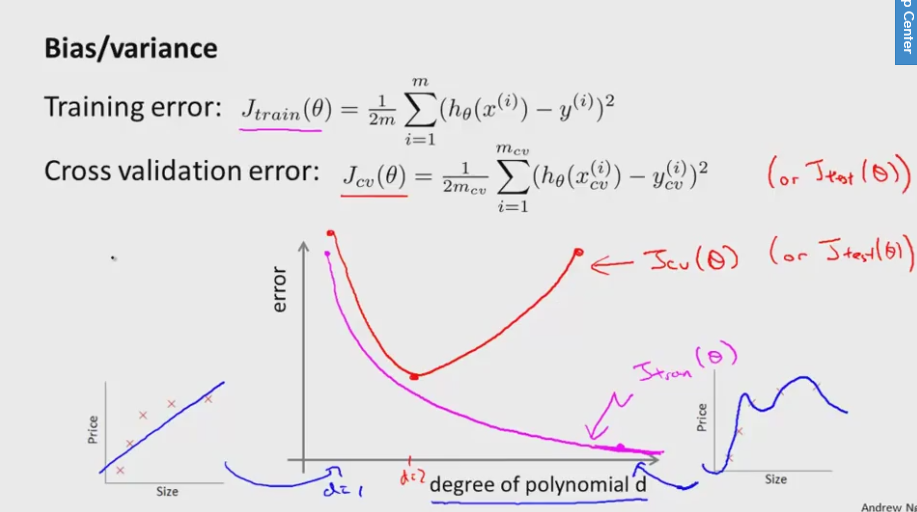
\includegraphics[scale=0.5]{sections/cs229/w7/bias_var.png}
	\end{center}

	\item High bias is shown on the left, where you have a low order polynomial with a large error
	\item High variance is shown on the right, where you have a high decree polynomial with a large error
	\item Your model suffers from high bias (underfit) problem if the training error is high and the cv is approximately the same.
	\item Your model suffers from high variance (overfit) if the training is low (fit well) while the cv error is much greater than the training error
\end{itemize}


\subsubsection{Regularization and Bias/Variance}
\begin{itemize}
	\item In regularization we have a regularization term with a variable $\lambda$
	\begin{center}
		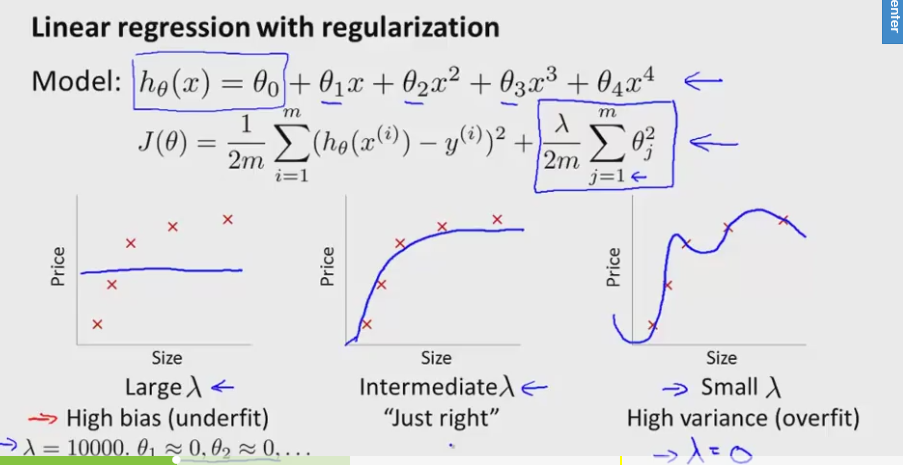
\includegraphics[scale=0.5]{sections/cs229/w7/reg.png}
	\end{center}

	\item When you have a large $\lambda$ all parameters are heavily penalized, so only the constant term remains
	\item Contrasting, when we have a small $\lambda$ we maintain our very high variance overfitting
	\item We want to find the ``just right'' value
	\item Choosing the regularization parameter $\lambda$
	\begin{itemize}
		\item Try multiples of $\lambda=0,0.01,0.02,0.04,0.08,\ldots, 10$
		\item Let the models of each value of $\lambda$ be $\theta^{(n)}$
		\item Choose the smallest $J_{cv}(\theta{(n)})$
	\end{itemize}

	\begin{center}
		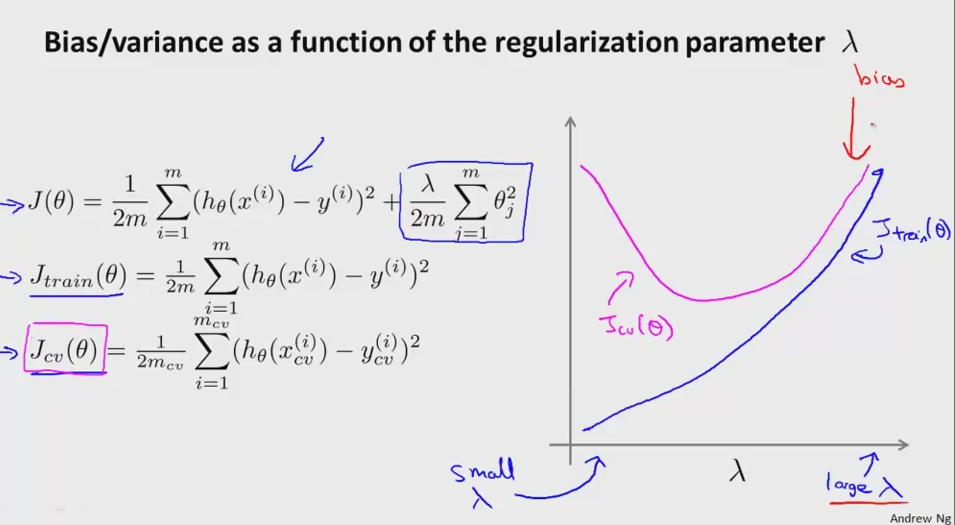
\includegraphics[scale=0.5]{sections/cs229/w7/lambda.png}
	\end{center}
	\item For small $\lambda$ you have little penalty and are able to fit your data well 
	\item The cross validation error is very high when $\lambda$ is small because you fit the too perfectly to other data set
\end{itemize}

\subsubsection{Learning Curves}
\begin{itemize}[--]
	\item Plot $J_{train}$ or $J_{cv}$ against $m$ (training set size)
	\item To do this we will deliberatly limit our training set size to complete the graph at lower points

	\item Suppose you have a high bais, If we were to increase the training set size you end up with a similar straight line
	\item The cv error will plateau out because the line can't conform any better to the data 
	\item The training set also has a similar error because it's unable to also conform to the data
	\item It has a high bias because both errors are high
	\item If a learning algorithm is suffering from high bias, getting more training data will not (by itself) help much.
	\begin{center}
		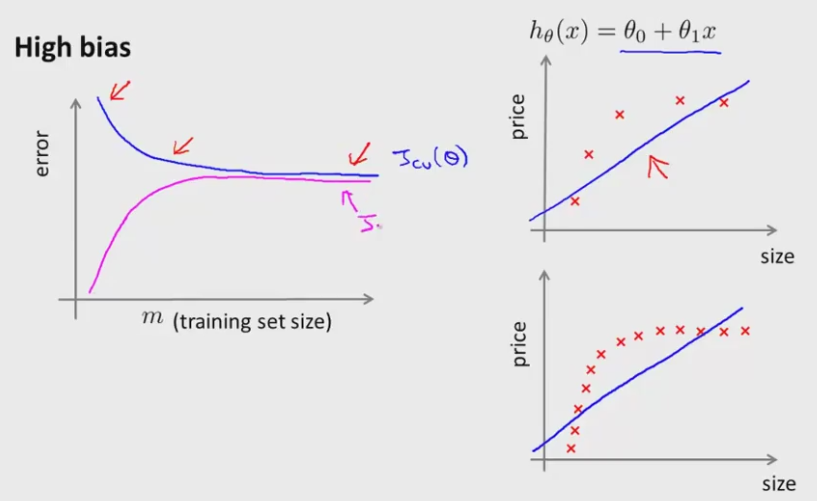
\includegraphics[scale=0.5]{sections/cs229/w7/bias.png}
	\end{center}

	\item Suppose now you have high variance, we will fit the data very well; however, it will largely overfit the data
	\item Since we can very easily fit the data our training error will remain low
	\item However, the cross validation error will remain high because it's too perfectly fitted for other data points
	\item The variance occurs do to this large gap in error between cv and training
	\item If a learning algorithm is suffering from high variance, getting more training data is likely to help.
	\begin{center}
		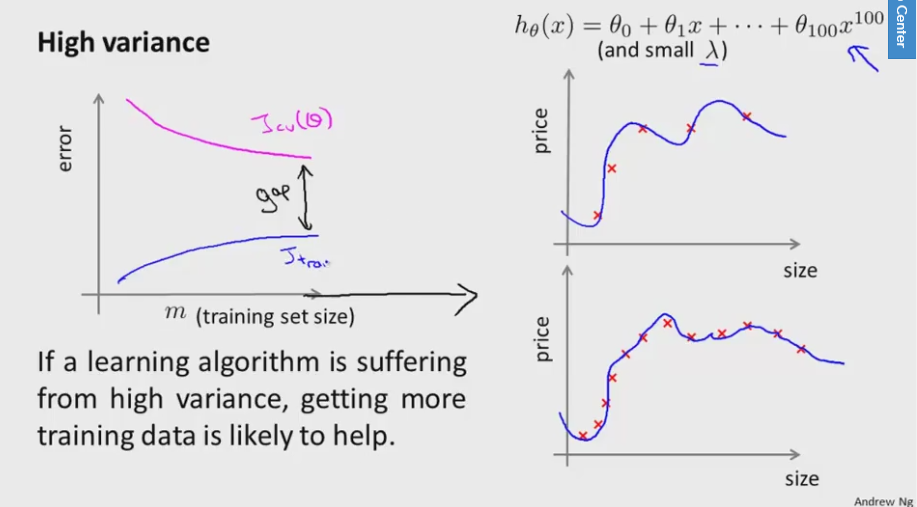
\includegraphics[scale=0.5]{sections/cs229/w7/var.png}
	\end{center}


\end{itemize} 

\subsubsection{Deciding What to Do Next Revisited}
\begin{itemize}[--]
	\item What should you try next?
	\begin{itemize}[--]
		\item Get more training examples $\to$ fixes high variance
		\item Try smaller sets of features  $\to$ fixes high variance
		\item Try getting additional features $\to$ fixes high bias (typically)
		\item Try adding polynomial features $\to$ fixes hih bias
		\item Try decreasing $\lambda$ $\to$ fixes high bias (less penalty for complex features)
		\item Try increasing $\lambda$ $\to$ fixes high variance (more penalty for complex features)
	\end{itemize}

	\item ``Small'' neural networks: fewer parameters; more prone to underfitting; computationally cheaper

	TODO: Draw

	\item ``Large'' neural network: more parameters; more prone to overfitting; computationally more expensive; use regularization to address overfitting

	TODO: Draw

	\item Try using the training/cv/test sets to determine the best choice for number of hidden layers
\end{itemize}
